\title{}
\documentclass[8pt]{memoir}
\usepackage[a4paper]{geometry}
\usepackage{multicol}
\usepackage[pdftex,bookmarks=true]{hyperref}
\usepackage{graphicx}
\usepackage{xcolor}
\usepackage{afterpage}

\newlength{\mylen}
\addtolength{\mylen}{\textheight}
\addtolength{\mylen}{-16pt}
\renewcommand{\familydefault}{\sfdefault}


\begin{document}
\newenvironment{changemargin}[2]{%
\begin{list}{}{%
\setlength{\topsep}{0pt}%
\setlength{\leftmargin}{#1}%
\setlength{\rightmargin}{#2}%
\setlength{\listparindent}{\parindent}%
\setlength{\itemindent}{\parindent}%
\setlength{\parsep}{\parskip}%
}%
\item[]}{\end{list}}


% Make one image take up the entire slide content area in beamer,.:
% centered/centred full-screen image, with title:
% This uses the whole screen except for the 1cm border around it
% all. 128x96mm
\newcommand{\titledFrameImage}[2]{
\begin{frame}{#1}
%\begin{changemargin}{-1cm}{-1cm}
\begin{center}
\includegraphics[width=108mm,height=\textheight,keepaspectratio]{#2}
\end{center}
%\end{changemargin}
\end{frame}
}

% Make one image take up the entire slide content area in beamer.:
% centered/centred full-screen image, no title:
% This uses the whole screen except for the 1cm border around it
% all. 128x96mm
\newcommand{\plainFrameImage}[1]{
\begin{frame}[plain]
%\begin{changemargin}{-1cm}{-1cm}
\begin{center}
\includegraphics[width=108mm,height=76mm,keepaspectratio]{#1}
\end{center}
%\end{changemargin}
\end{frame}
}

% Make one image take up the entire slide area, including borders, in beamer.:
% centered/centred full-screen image, no title:
% This uses the entire whole screen
\newcommand{\maxFrameImage}[1]{
\begin{frame}[plain]
\begin{changemargin}{-1cm}{-1cm}
\begin{center}
\includegraphics[width=\paperwidth,height=\paperheight,keepaspectratio]{#1}
\end{center}
\end{changemargin}
\end{frame}
}
\newpage

%changing the page design temporarily
\changepage{9cm}{9.4cm}{-4.7cm}{-4.7cm}{}{-4.5cm}{}{}{}
%\noindent\rule{\textwidth}{\textheight}
\includegraphics[width=\textwidth,height=\textheight]{haeckelmap}
\newpage

%restoring the standard settings
\changepage{-9cm}{-9.4cm}{4.7cm}{4.7cm}{}{4.5cm}{}{}{}

%\newgeometry{left=0cm,top=0cm,right=0cm}
%
%\maxFrameImage{haeckelmap}
%\pagecolor{gray}\afterpage{\nopagecolor}
%\clearpage
%
%\newpage
%
%%\begin{figure}[!ht]
%% \parbox[t][\mylen]{\textwidth}{%
%% \centering
%% \includegraphics{haeckelmap}
%%
%% \vfill
%% \caption{World Map}
%% }
%%\end{figure}
%
%\restoregeometry

\chapter{Character Creation}\label{chargen}
\pagecolor{gray}\afterpage{\nopagecolor}



\newpage
\pagecolor{gray}\afterpage{\nopagecolor}
\fontfamily{pzc}
\selectfont
%\begin{figure}[h]
%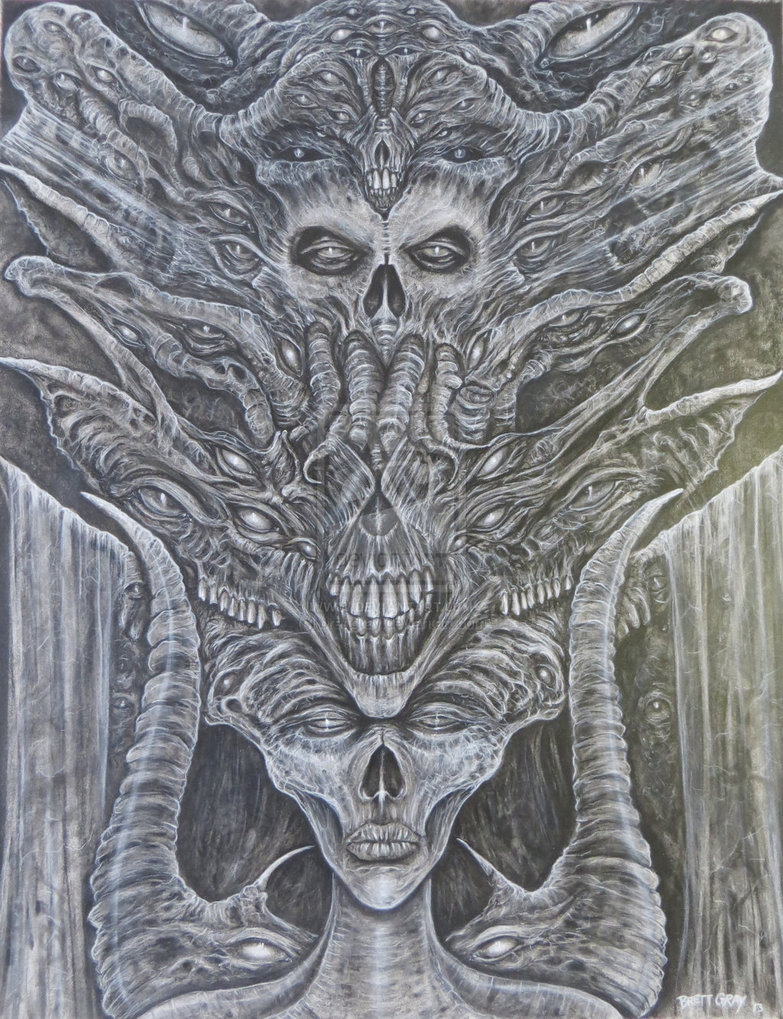
\includegraphics[scale=0.3]{priestess}
%\end{figure}
Birds chirp and the sounds of a flute hum in the atmosphere. The party comprises of Maden Rak, Exeter and Victoria. They travel through the Violet Forest to the Town of Bodmin. 

``Do you hear that?'' 

``I smell Elf.''

On a tree sits an Elf playing a flute. He is fully donned in black and brown leather armour. Over his face is a bandana. His pointed ears stand out prominently. 

``That is...'' before being interrupted by the Elf.

``Maden Rak. Special Forces Commander of the Midgaardian Roaches. Servant of the Dark. Hunter of Elves, murderer of women and children. Twice decorated for valour on the field of battle.'' He claps.

``Caeryn, son of a whore.''

``I've long awaited our meeting. Laid plans, set traps... And now you appear in my forest of your own volition.''

``We are here to bring to justice the Kingslayer and those who aid him. You will rot in a Midgaardian jail!''

``Good luck. This is our land. You will not win here.''

``Since when did the Elves hire professional killers to do their dirty work. The Elves have fallen low.''

``King or beggar, whats the difference? One Human less.''

``Dont make a big deal of the race thing.''

``Yet race is the very reason we fight! We have pointed ears, you have rounded. We have long lives, you have short. Yet you multiply quickly, like vermin, but die just as easily.''

``This is not about race, or freedom, or vengeance. You just refuse to see the obvious truth.''

``And what is that obvious truth?''

``That you are just being used by others.''

``That was a thing of the past! We shall not be used again.''

``Enough of this piss!'' Maden Rak throws a knife at the Elf, who then dodges clumsily in surprise, regains his footage, and then runs up to higher ground using the cover of archers. 
\normalfont

\newpage
\begin{multicols}{2}
This chapter goes through the process of creating a character in the world of Haeckel. There three ways of making characters. 

The basic method that is faster but has reduced options. I chose to build this system so that GMs could use it to help people quickly make characters on the fly such as when GMing in real life with a new gaming group. In this situation you often dont have the time to spend an hour (or more) on character creation.

It makes a party of Humans that are relatively skilled - being of the 1st level.   

And the advanced method which takes abit longer (and involves some reading) but more options. 

Characters built using either system are pretty much the same power level so the only key factor when choosing which to use is how much time you wish to spend making your character. 

The final system is the 0th level system. It makes a party of characters that are trained in a profession but not in adventuring. This system is for relatively mundane characters to be thrown in over their heads in some dire situation, as the GM requires. 

\section{Basic System 1st Level}

\begin{enumerate}
    \item The ability scores are: Strength (STR), Dexterity (DEX), Constitution (CON), Intelligence (INT), Wisdom (WIS), and Charisma (CHA). Record these down using the short hand version in brackets. 
    \item Roll 4d6 drop lowest for each ability score. Check the table below to see the 'ability score modifiers'. This number is based off your Ability Score and is the number that affects your dice rolls. 
    \item In the Basic System you default to a Human. Pick any Ability Score and increase it by +2.  
    \item Choose your class. Your options are: Fighter (STR), Wizard (INT), Rogue (DEX) and Cleric (WIS). Read the page on Core Classes. If you are a beginner player I highly suggest picking the Fighter class; however the Rogue and Cleric are okay for beginners too. I suggest only picking the Wizard class if you are an experienced player or want an additional challenge.
    \item Choose two ability scores to be Primary Attributes (this includes the bonus from being Human, as most other races would only get a choice of 1 Primary Attribute. Your class determines your third Primary Attribute. Your Primary Attributes represents the type of tasks you are best at solving while under pressure or with immense risk, and thus in a significant way shape the kind of character you have.
    \item Pick one equipment starting package. They are described below. Make a note of how much the package weighs. 
    \item You now need to calculate Carrying Capacity. This is equal to your Strength Ability Score. If Strength is your Primary Attribute you gain an additional +4. Likewise, if Constitution is one of your Primary Attributes you gain an additional +4 (stacking with the Strength bonus). For example, a Character with 16 Strength, and has a Primary Attribute of Str AND Con would have a carrying capacity of 24 (16+4+4).
\end{enumerate}

\begin{tabular}{l | r}
    Ability Score & Ability Modifier \\
    \hline
    18 & +3 \\
    16-17 & +2 \\
    13-15 & +1 \\
    9-12 & 0 \\
    6-8 & -1 \\
    3-5 & -2 \\   
\end{tabular}

%\begin{tabular}{l | c | r }
%Fighter Archetypes & Package & Space \\
%\hline
%Swordsman & Blah & 0 \\
%Archer & Blah & 0 \\
%Pikeman & Blah & 0 \\
%Axewielder & Blah & 0 \\
%\end{tabular}
%
%\begin{tabular}{|p{1.5cm}|p{5cm}|p{1cm}|}
%Rogue Archetypes & Package & Space \\
%\hline
%Lovable Rogue & Blah & 0 \\
%Burgler & Blah & 0 \\
%\hline
%Thug & Blah & 0 \\
%\hline
%Explorer & Crossbow, case with 20 bolts, short sword, 2 throwing daggers, sturdy leather armor, tanned brown cloak, thick tunic and pants, leather belt, low boots, backpack, 2 large treasure sacks, 50' rope, tinderbox, lantern, small hammer, 12 iron spikes, 2 flasks of military oil, wineskin, 2 weeks’ iron rations, 3gp & 0 \\
%\hline
%\end{tabular}
%
%\begin{tabular}{l | c | r }
%Cleric Archetypes & Package & Space \\
%\hline
%Priest & Blah & 0 \\
%Crusader & Blah & 0 \\
%Inquisitor & Blah & 0 \\
%Witch Hunter & Blah & 0 \\
%\end{tabular}
%
%\begin{tabular}{l | c | r }
%Wizard Archetypes & Package & Space \\
%\hline
%Witch & Blah & 0 \\
%Scholar & Blah & 0 \\
%Hedge Mage & Blah & 0 \\
%Monk & Blah & 0 \\
%\end{tabular}

\section{Advanced System 1st level}

\begin{enumerate}
    \item The ability scores are: Strength, Dexterity, Constitution, Intelligence, Wisdom, and Charisma. 
    \item Roll 4d6 drop lowest for each ability score.
    \item Choose your race. This may affect your ability scores. 
    \item Choose your homeland, and background.
    \item Choose your class. You can pick from any of the Core Classes or Campaign Classes. Your MAX HP is determined by your class choice and current Constitution ability modifier.
    \item Pick one sphere as your primary sphere.
    \item Pick one feat. The flaws are for more experienced players who would like an additional challenge.
    \item Choose your equipment. For fast play choose a starting package.
    \item Optionally pick a deity to follow. 
    \item Optionally choose a Faction that you aspire to join. 
    \item Optionally choose an Important Character for your character to know about and may want to be involved with. 
\end{enumerate}


\section{0th Level}

\begin{enumerate}
    \item Roll 3d6 for each ability score: Strength, Dexterity, Constitution, Intelligence, Wisdom, and Charisma.
    \item Roll 1d4 for health points, and add your Constitution modifer, as seen in the table above.
    \item Roll on the profession table to randomly determine your profession. This also determines your starting items.
    \item Choose your race. 
    \item Choose 1 ability score to be your Primary Attribute. Or choose 2 ability scores if you are a Human. 
\end{enumerate}

The way this works is basically: if a character survives the first adventure, they become a 1st level character. They may choose a class as per the usual rules. The weapon they used most during the adventure is the weapon they are proficient with at 1st level - unless they're a fighter, in which everything is proficient. 

\end{multicols}


\chapter{Core Classes}\label{coreclasses}
\pagecolor{gray}\afterpage{\nopagecolor}
\newpage
\pagecolor{gray}\afterpage{\nopagecolor}
\fontfamily{pzc}
\selectfont
Co-Consul of Ablon enters the Office and the General Autorius sits at his table, golden goblets of wine and a plate full of grapes rests easy in front of him. 

``We had an agreement, that we'd share all revenue.''

``Yes''

``Hereopolis has agreed to give you 20,000 pounds of gold. I want my share.''

``Who told you this?''

``You deny?''

``Who told him.''

``I have spies among his people.''

``If Herod is kind enough to give me a gift, what business is it of yours? A gift is not revenue.''

It is not a gift, it is a bribe. For political and military favours. The cost of which favours shall be born by the state.''

``Peasantry.''

``Let us be realistic. This arrangement of ours can not work if you seek every opportunity to aggrandize yourself at my expense.''

``Laughter. Aggrandize myself. This from the boy whose so called father has been declared a God.''

``An honour he well deserves.''

``You only did it so you might be known as the Son of a God. You have no accomplishments of your own, so you seek to borrow the glory of others.''

``Its true, it was no accomplishment to defeat you at Mutina.''

``You defeated me? You cowardly little shit. You never left your tent. You have never defeated me, in anything.''

``Gentlemen, lets not get overheated. Im sure we can come to some reasonable agreement. I had hoped that you had learnt some humility and discipline. You are still the same old crude, arrogant, lech that you always were.''

``Thats right. Just the same. The same that is still fucking your mother!''
\normalfont
\newpage

%changing the page design temporarily
\changepage{9cm}{9.4cm}{-4.7cm}{-4.7cm}{}{-4.5cm}{}{}{}
%\noindent\rule{\textwidth}{\textheight}
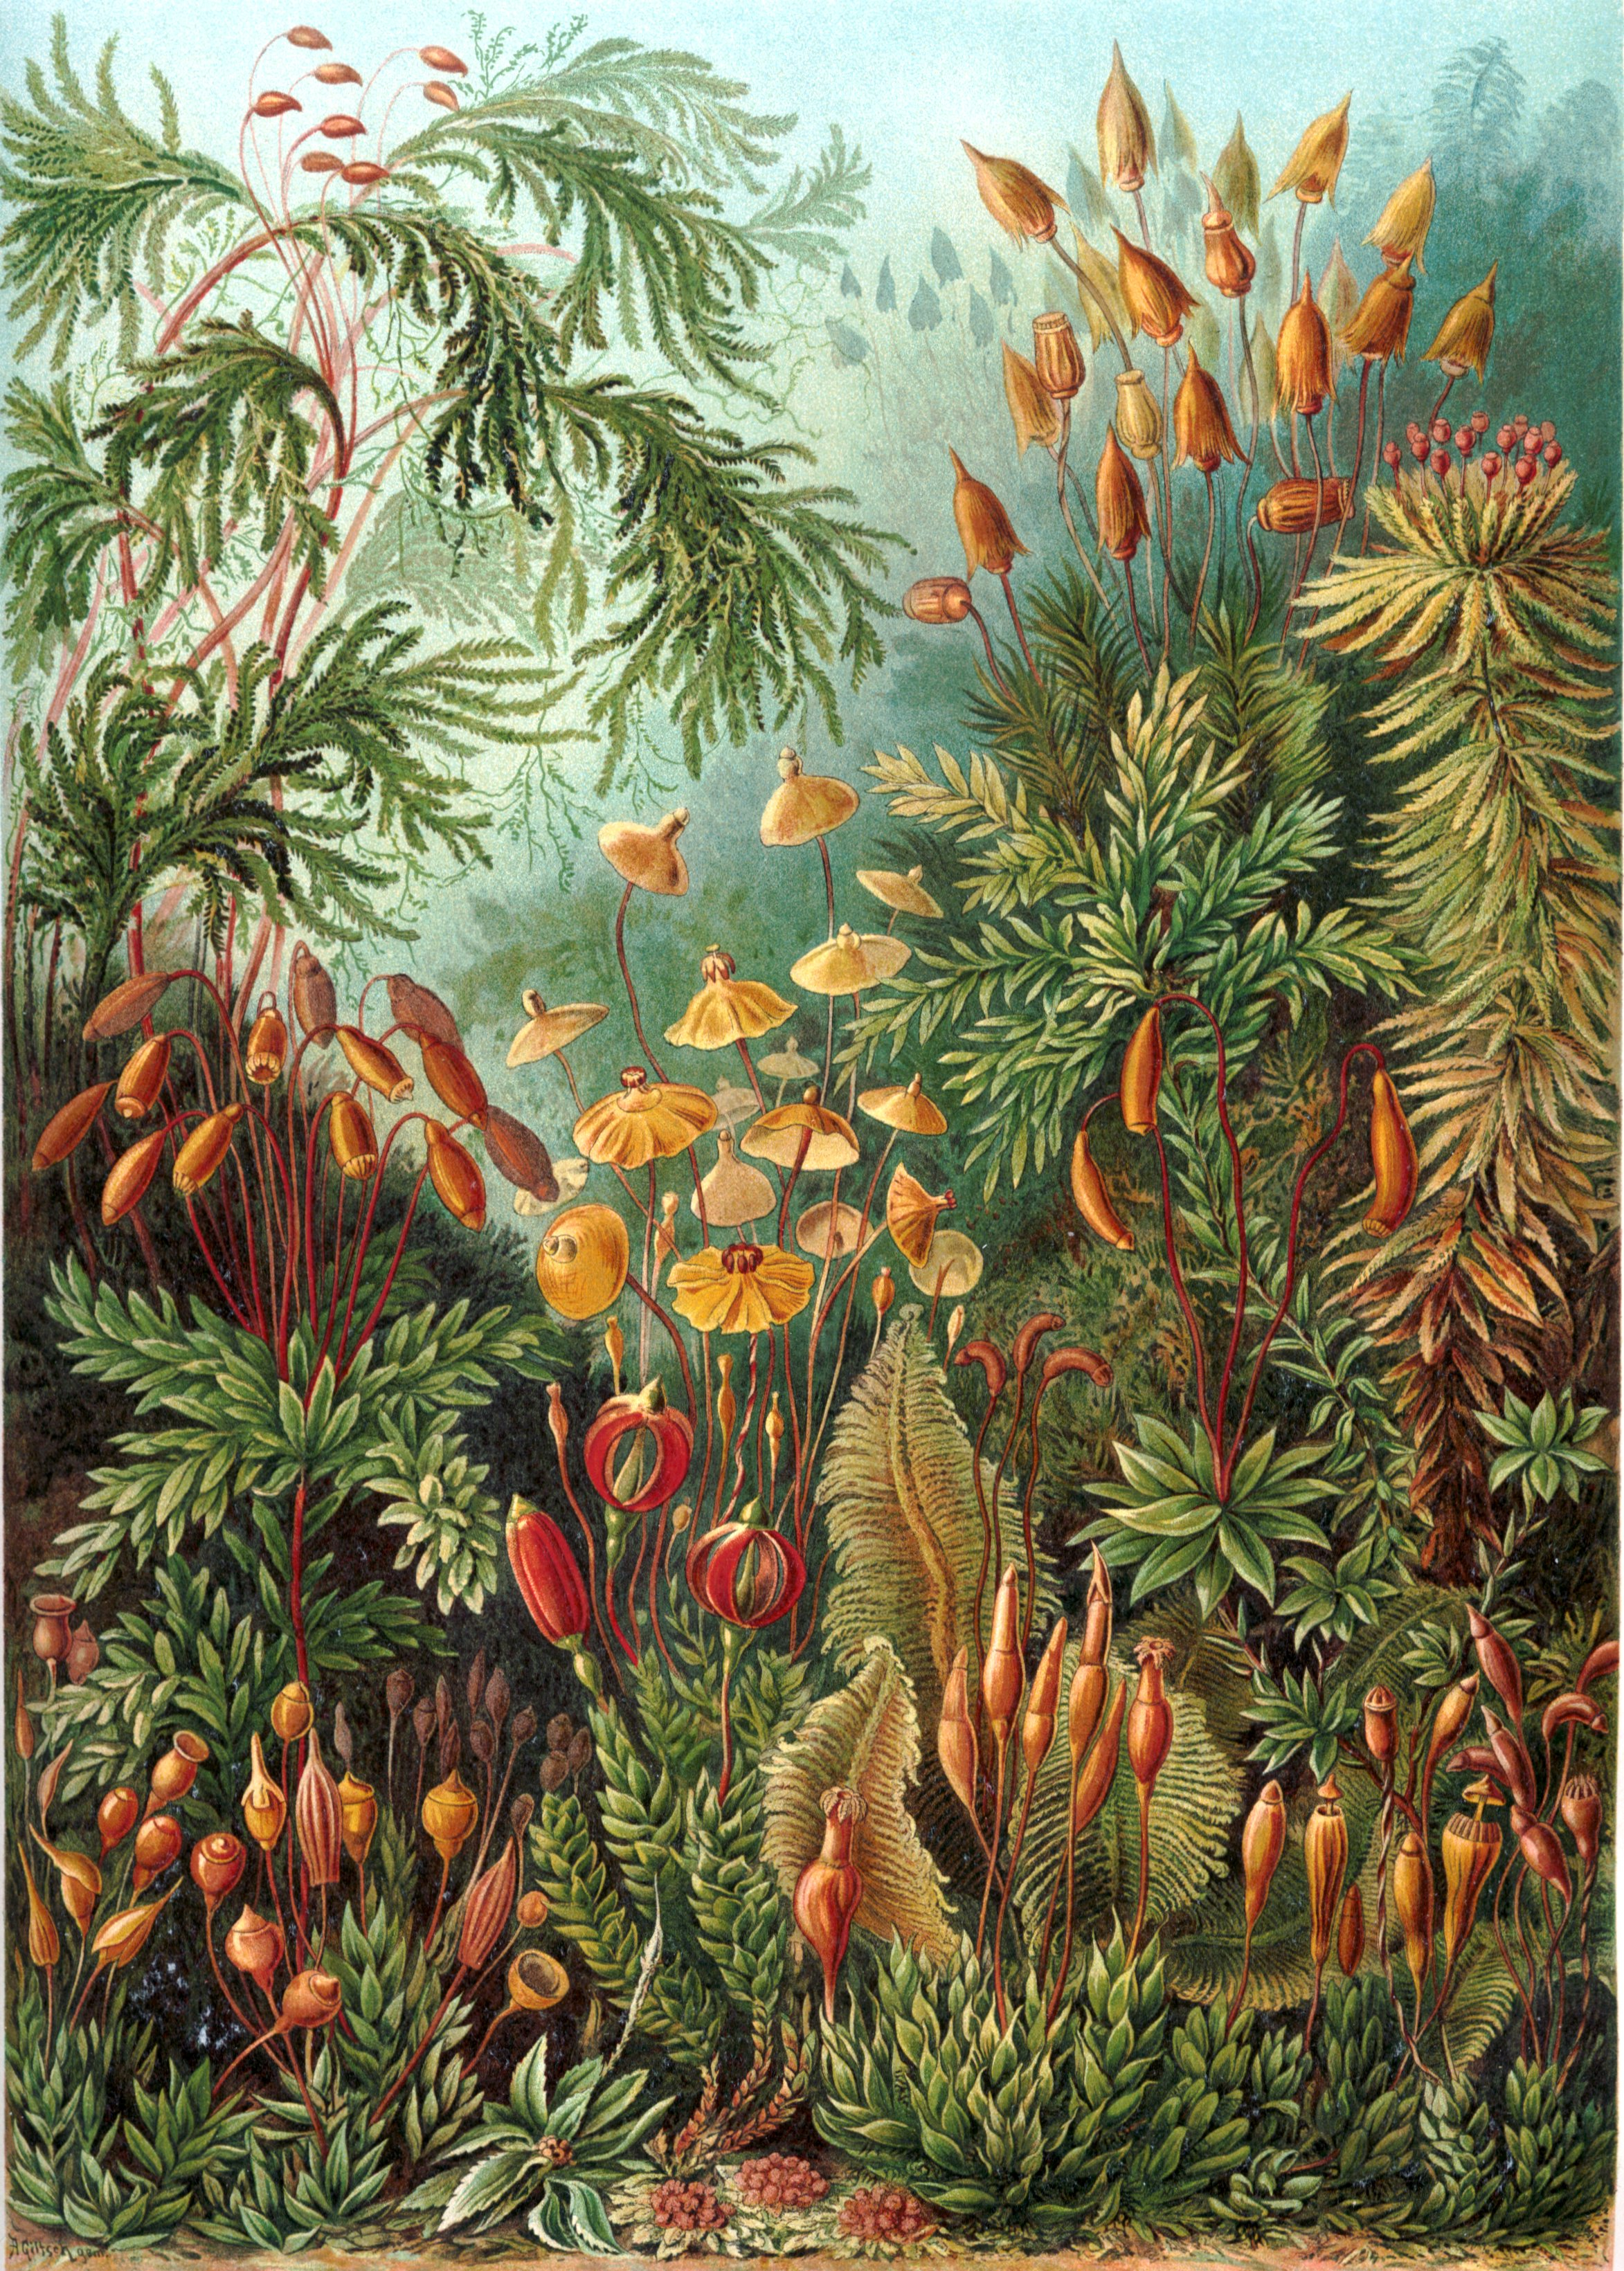
\includegraphics[width=\textwidth,height=\textheight]{Haeckel_Muscinae}
\newpage

%restoring the standard settings
\changepage{-9cm}{-9.4cm}{4.7cm}{4.7cm}{}{4.5cm}{}{}{}

\begin{multicols}{2}
The Core Classes are archetypical classes to the worlds most popular RPG system. They encapsulate problem solving philosophies and a way of playing the game. 

This class system is designed to be extremely simple. It is fundamentally an "open formed gaming" system. I.e. pretty much every character can sneak around, or swim, or climb walls. The difference is that certain characters have additional capabilities above the norm. 

It is very fine to have an entire party composed of Fighters. Having a cleric on the team greatly increases survivability however. 

\section{Fighter} This class is best at solving problems via brute force. They are not just a duelist but are skilled in any form of warfare. 

The Fighter may use any weapon or armour. Their starting HP is 10. Each time they level up they must roll 1d10 to determine the HP gained for that level up. This makes them a very tough class to kill relative to the other classes.

The Fighter class is illiterate but can speak in Common.  

\section{Wizard} They are the late game class. Their starting HP is 4, and they gain 1d4 hp per level up. Most wizards are proficient with no weapons and armour, unless some other mechanic such as Race dictates otherwise. To survive you will have to master using terrain and keeping aware of your surroundings. 

The capabilities of the Wizard are virtually unknown. They are an esoteric class whom start off as a Scholar without spellcasting capabilities and must learn dark secrets to unlock their potential. They are thus not suitable for brief adventures and best suited for campaign play.

As a Wizard you begin knowledgeable in one of the fields of Academia. You have two basic ways to use this. You can ask the GM for advice or information pertaining to the topic, and/or you can use your own knowledge of the topic (relevant to the time period of the game) to your own advantage. 

The Wizard class begins literate in Common and High Common - the language of the nobility classes.  
 
\section{Rogue} Rogues may only wear leather armour and are severely limited in their weapon selection. The most common rogue weapons are Daggers and Shortbows. Their starting HP is 4 and they roll 1d4 each time they level up for extra HP. The rogue class has access to a number of special skills that provides them additional utility. 

Their two principal combat abilities are Backstab and Set Traps. Their utility abilities are: Hide in Shadows, Climb Steep Slopes, and Listen at Doors.

The Rogue class is illiterate but can speak in both Common and Low Common - the language of the criminal underworld. 

\section{Cleric}

Clerics may wear armour and use any weapon. Their starting HP is 8 and they roll 1d8 each time they level up for extra HP. 

The principal advantage of playing a Cleric is that of your involvement with society at large. If you have a local congregation, it is likely that they will come to your aid, and it is expected that you come to theirs in times of need. 

Some Churches become extremely powerful allies. Also, ostensibly, merchants are less willing to rip off Clerics than other classes. This is not a fool proof way of being safe from scams however.  

The Cleric class can read and write in Common and Gothic - an ancient language of religious scripture.

\end{multicols}

\chapter{Equipment}\label{equipment}
\pagecolor{gray}\afterpage{\nopagecolor}
\newpage
\pagecolor{gray}\afterpage{\nopagecolor}
\fontfamily{pzc}
\selectfont
In the Midgaardian Keep, Castle Black, a young noble Lord aged 11 lays in bed. His servant, a short lady who has seen many years sits in a chair on the opposite side of the room. She knitts a scarf with delicate and refined movements. 

``Have I ever told you that my pappy fought in the Great War? It was a long time ago, your parents had'nt even been born yet.''

``I dont like those kind of stories. Knights in shining armour are not my thing.''

She chuckles, ``So what kind of stories do you like my little Lord.''

``The scary ones.''

``The Great War was scary my little Lord! It wasn't a romance tale like your sages say. 'The Days of Dread' - that's what we called life back then. There were no goodly kings then, no no. One House was composed of vile necromancers!''

``The Mordenheims? I read a bit of them, but my teachers constantly change the topic when I inquire further.''

``We didn't know them by their names then, young Lord, but we knew what they did. Long after the war had ended, Pappy would wake up in the night sometimes screaming. When I was grown I finally asked him why that happened, and he said: 'Every time I sleep I see my brother. But not... like you knew him, Helga. I see him when he was killed. And I see him when he rose again, and I see him when he tried to strangle me with his cold, dead hands. And finally, I see his walking corpse's head sliced clean off by my commander.' ''

The little Lord rests his head on his silk pillow. On his fair and normally jaded face curls a small smile. 

\normalfont
\newpage



\section{Simple Exploration Logistics}

\begin{tabular}{l l l l l }
    Type & Desc & Lasts & Cost & Weight \\
    \hline
    A & Basic Excursion & 3 days & 25 gp & 30lb \\
    B & Extended Excursion & 7 days & 50 gp & 75lb \\
    C & Prolonged Excursion & 14 days & 120gp & 140lb \\
    D & Basic Dungeon Crawl & 1 day & 50 gp & 50lb \\
    E & Extended Dungeon Crawl & 3 days & 100 gp & 85lb \\
    F & Basic Overland Excursion & 2 days & 35 gp & 50lb \\
    G & Extended Overland Excursion & 7 days & 80 gp & 100lb \\
\end{tabular}

\begin{framed}\centering
The purpose of this system is for campaigns where resource management or the specific use of inventory items is simply a distraction and is heavily de-emphasised in that scenario. For verisimilitude purposes you can say that due to wear and tear the items in the kit simply are heavily damaged, muddy beyond use, or whatever.  
\end{framed}
\begin{multicols}{2}
\section{Starting Equipment Sets}

\subsection{Brouliard}

\paragraph{Socialite} Small dog familiar, long slender sword, stiletto, form-fitting chain mail armor, silvery white silk cloak and sapphire blue dress, tear-drop silver earrings (10gp value), high boots, 2 purses, 1 week’s iron rations, 31gp

\paragraph{Dilettante} Slightly notched short sword, dagger, leather armor, shabby linen tunic and pants, leather belt, low boots, belt pouch, pair of dice carved with leaves, 1 week’s iron rations, 3gp

\paragraph{Intriguer} Composite bow, quiver with 20 arrows, long slender sword, stiletto, light steel shield, form-fitting chain mail armor, midnight blue cloak embroidered with silvery, midnight blue cassock, high boots, backpack, 34gp.

\paragraph{Swashbuckler} Shortbow, quiver with 20 arrows, scimitar, 2 well-balanced daggers with boot- sheathes, leather armor, colorful tunic and pants, bright silk girdle, high boots, wineskin with good wine, small sack, 50' rope, grappling hook, 1 week’s iron rations, 7gp.

\paragraph{Aristocrat} Crossbow, case with 20 bolts, matching sword and dagger with lacquered hilts, exquisitely stitched leather armor, fur-lined cloak, armiger’s tunic and pants, embossed leather belt, high boots, medium riding horse, riding saddle and tack, saddlebags, 1 week’s iron rations, 20gp

\paragraph{Bounty Hunter} Bola, serrated sword, dagger, net, leather armor, black cloak, traveler’s tunic and pants, high boots, backpack, crowbar, 50' rope, manacles, 12 iron spikes, small hammer, 2 weeks’ iron rations, 2gp.

\paragraph{Cutthroat} Hand axe, dagger, leather armor, cheap tunic and pants, leather belt, low boots, backpack, 12 iron spikes, small hammer, 1 flask of military oil, tinderbox, 12 torches, 2 weeks’ iron rations

\paragraph{Merchant Traveller} Crossbow, case with 20 bolts, short sword, 2 throwing daggers, sturdy leather armor, tanned brown cloak, thick tunic and pants, leather belt, low boots, backpack, 2 large treasure sacks, 50' rope, tinderbox, lantern, small hammer, 12 iron spikes, 2 flasks of military oil, wineskin, 2 weeks’ iron rations, 3gp

\paragraph{Nessian Vikingr} Bearded Longaxe, painted wooden shield, woolen cloak, iron helmet, NOT COMPLETE. 

\subsection{General} 
\paragraph{Abloni Free Gladiator} Gilded sword, large steel shield, lamellar armor, plumed heavy helmet with visor and crest, leather cloak, loincloth, high sandals, backpack, amphora of oil (for polishing body), 2 weeks’ iron rations, 15gp in arena winnings

\paragraph{Hunter} Sturdy longbow, quiver with 20 arrows, leaf- headed spear, gracefully curved short sword, dagger, chain mail armor, wind-battered fur cloak, wool tunic and pants, leather belt, low boots, backpack, lantern, tinderbox, 2 flasks of common oil, blanket, 50' rope, 12 iron spikes, small hammer, wineskin, 1 week’s iron rations

\paragraph{North Wall Death Dealer} Two-handed iron sword, francisca, chain mail armor, wool tunic and pants, leather belt,
low boots, silver arm-bands (25gp value), wineskin with strong ale, small sack, 50' rope, grappling hook, 2 weeks’ iron rations, 1gp

\section{Equipment Kits} 

\begin{framed}\centering
The purpose of these are to speed up the purchasing process as well as making it obvious to new players the kinds of items they will need.  
\end{framed}

\paragraph{Kit, Infiltration; Price 140 gp; Weight 15 lbs;}

This kit is useful to adventurers who must practice guile and deception in order to acquire useful information, and includes a set of caltrops, chalk, a disguise kit, an ear trumpet, fake footprint shoes, a skeleton key, and a wrist sheath. For Small creatures, the weight of an infiltration kit is 9 pounds.

\paragraph{Kit, Gear Maintenance Price 5 gp; Weight 2 lbs.}
This kit contains metal polish, a small file, a leather paring knife, conditioning oil for leather, two soft cloths, extra leather straps, a sewing needle, and a few buttons.

\paragraph{Kit, Grooming; Price 1 gp; Weight 2 lbs.}
This pouch of toiletries includes a comb, scissors, a nail file, a sponge, a hairbrush, a miniature mirror, soap, a chewing stick, and tooth powder.

\paragraph{Kit, Fighter's; Price 9 gp; Weight 29 lbs.}
This kit includes a backpack, a bedroll, a belt pouch, a flint and steel, an iron pot, a mess kit, rope, soap, torches (10), trail rations (5 days), and a waterskin.

\paragraph{Kit, Cooking; Price 3 gp; Weight 16 lbs.}
This kit contains an iron pot, an iron skillet, a ladle, a skewer, a wooden cutting board, a cutting knife, an iron tripod for the pot, a packet of tinder, and a small selection of local or otherwise easy to find seasonings. You can attach the skewer to the tripod for roasting small game animals. All the component pieces (except the skillet) fit within the pot for easy storage and transport.

\paragraph{Kit, Cleric's; Price 16 gp; Weight 32 lbs.}
This includes a backpack, a bedroll, a belt pouch, candles (10), a cheap holy text, a flint and steel, an iron pot, a mess kit, rope, soap, a spell component pouch, torches (10), trail rations (5 days), a waterskin, and a wooden holy symbol.

\paragraph{Kit, Campsite; Price 12 gp; Weight 80 lbs.}
This kit is actually four bundles of gear, designed so four individuals can share the load. It consists of four bedrolls, four blankets, a day's worth of firewood, a flint and steel, a tindertwig, four mess kits, a cooking kit, and 8 days of trail rations (with the expectation that adventurers will supplement the rations with a little hunting as they travel). Adventurers expecting inclement weather should also purchase one or more tents.

\paragraph{Kit, Breaker's; Price 353 gp; Weight 40 lbs.}
This kit contains all manner of items useful for smashing down doors, creating diversions, and blowing things up. It includes a dose of alchemist's glue, a flask of alchemist's fire, a crowbar, a drill, a fuse grenade, a glass cutter, a jetcaster, a vial of phosphorescent gel, 4 pints of oil, a portable ram, a dose of rusting powder, 5 tindertwigs, and a wire.

\paragraph{Kit, Riding; Price: 16gp; Weight 54 lbs.}
This kit includes a bit and bridle, a saddle, a saddle blanket, saddlebags, and 2 days' worth of feed for a mount. The weight can be lightened 10 pounds by discarding the feed.

\paragraph{Kit, Rogue's; Price 50 gp; Weight 37 lbs.}
This kit includes a backpack, a bedroll, a belt pouch, caltrops, chalk (10), a flint and steel, a grappling hook, an iron pot, a mess kit, a mirror, pitons (10), rope, soap, thieves' tools, torches (10), trail rations (5 days), and a waterskin.

\paragraph{Kit, Gypsy Signal Kite}

Gypsies are a strange lot. Given that they travel and do not rely on societies messenger systems they have needed to develop their own way of communicating with each other. To this end they invented signal kites. Built from paper glued to bamboo frames, their kites are painted with various colors and pictures. In addition to flying kites as a leisure activity, gypsies also fly kites of various shades and patterns to send signal messages. Gypsies have developed an extensive code of signals and can use their kites to display complex messages visible at great distances. A signal kite kit includes six small colored kites that can be hooked together in different patterns to facilitate complex messages. The kit also includes a spool and 300 feet of twine. Sending or interpreting a signal kite's message requires understanding the Gypsy language.

\paragraph{Kit, Trapper's; Price 263 gp; Weight 90 lbs.}

This kit is particularly useful for dungeon explorers who specialize in trapping or taming whatever vile quarry they find. A trapper's kit contains an average lock, a bear trap, a container of bone paste, a Small cage, a set of manacles, a bag of marbles, 50 feet of silk rope, two tanglefoot bags, 50 feet of twine, and a wire.

% Marching
% Combat
% Infiltration
% Siege
% Encampment
% 

\end{multicols}

%\section{Fashion}
%\subsection{Ablon}
%\subsection{Abyssimiar}
%\subsection{Brouliard}
%\subsection{Midgaard}
%\subsection{Nes}
%\subsection{Ubris Furor} 

%\section{Design}
%Haeckel's vastness and social problems leads it to having differing levels of technological advancement from region to region. While Humanity dominate the continent it must be said that some of the most advanced technologies were in fact developed by demi-humans. As it currently stands, Elven and Dwarven Technology is superior to Humankind's; however the Megacity State of Ablon's technology is fast catching up and can be said to be superior in some regards. Most demi-human technology has been lost to the centuries, and what remains have their craftsmanship as closely guarded secrets that they would take to the grave. 
%
%\begin{framed}\centering
%Haeckel eschews the notion of wealth to level balancing. We have chosen to take this approach because it reduces the "resource optimisation problem" that you have in many systems. For example, if you give player's 20 points to spend on something, they will aim to allocate it efficiently. This is the problem that causes a lot of very interesting magical items to rarely be used - because wealth is a limited resource that is literally capped to ones level. You break that coupling and you open up new possibilities.
%\end{framed}
%\section{Gear Sets}
%
%The purpose of this section is to speed up character creation and the purchasing of large bulks of items by creating packages that players can rapidly pick to suit their various purposes. 
%
%\section{Potions}
%efefef
%\section{Scrolls}
%    \paragraph{Scroll of Magic Mapping} Scrolls of magic mapping are Scrolls that, when read, reveal part of or the entire level map (if blessed) to the player.\section{Books}
%    \begin{snugshade} "Spacing between words did not exist until the 7th century. This facilitated reading for monks who were not familiar with High Gothic. However, the use of spaces between words did not become commonplace before the 12th century. It has been argued that the use of spacing between words shows the transition from semi-vocalized reading into silent reading." -- Codex of Old Literature by Julius Toronicus. \end{snugshade}
%    
%    \subsection{Tome} A tome is a large book, especially one volume of a multi-volume scholarly work.
%        \paragraph{Summa Theologica} An Ancient Tome on the subject of Midgaardian Theology. It is one of the classics of Haeckel and one of the most influential works in that region. It is a major work and a lofty read at 3500 pages. The original text Summa Theologica Prime is considered a Holy Relic.
%    \subsection{Journal / Ledger}
%    \subsection{Codex / Tablet} Predominantely from Ablon.     
%    \subsection{Treatise}
%    \subsection{Papyrus Scroll} Predominantely from Abyssimiar and the Southern Continent.
%        \paragraph{The Creation Myth} 
%    \subsection{Atlas}
%        \paragraph{Atlas of the World} A rare and most visually compelling volume. Produced to the highest standards of the day by the leading mapmaker of the day. It is a clear, detailed, and intricate work of art. For each area there is an accompanying text, giving sources and authorities for them. It is a dense work and it takes awhile to read. 
%        
%        A sufficiently intelligent and literate character can use this book to, in a sense, ask the GM questions on the geography of the world. The answers do not have to be 100\% accurate but they are usually a good answer. To use this, it takes time (between 1-6 turns) to find the answer. The volume is heavy and thus cannot be easily carried onto adventures.  
%\section{Lighting}
%\section{Food}
%\section{Weapons}
%    \paragraph{Quick Dagger} This blade shimmers in a hyper active and accelerated matter. Legend speaks that it bestows upon the wielder amazing speed and alacrity. Thieves across the entire world covert this blade and very few of it exist.  
%\begin{framed}\centering
%This is the best known weapon for the Rogue class. The only way to get this blade is to steal it. Thus creates a shadowy conflict where treacherous individuals do whatever they can to acquire it and hold onto it long enough to profit highly from it.     
%\end{framed}        
%
%\paragraph{Bow of Light} Charges arrows with sacred light. The arrows will only harm those with evil in their heart. It will never harm those with good in their heart; the logical implication being that you can fire it safely at an opponent engaged in melee combat with a Paladin. The arrows charged with light emit it for a duration of 1 turn (10 minutes); thus it serves as a multi-purpose tool.
%
%\section{Armour}
%\section{Jewelry}
%\section{Wands}
%\section{Rods}
%\section{Staves}
%\section{Pets}
%\section{Navalcraft}
%\section{Tool}
%    \paragraph{Waterproof Blanket} Waterproof blankets will, while in the players' inventory, completely protect all inventory items from rusting and water damage. Note that worn items are not protected by waterproof blankets.
%    \paragraph{Hooded Cloak} Protects worn items from water damage - though not from full immersion in water. Thus, it would be effective vs heavy rain, but not vs a water trap or a flash flood. 
%
%\section{Unorganised}
%\paragraph{Prosthetic Limb}
%
%\paragraph{Mercy Giver} 
%\paragraph{Battle Gorget} This throat protector consists of a metal throat-shield and overlapping, neck-encircling plates that are attached to a leather belt. It protects the wearer from strangulation, death by hanging, and stabbing or piercing damage done directly to the throat. The voice of those whom wear this mask seems to echo and become a pitch rougher which makes them more intimidating.
%\paragraph{Bone Mask} This skull-face mask is fashioned from bone from any source – with the only limitation being that the pair that is created must be from the same litter of animals. The powdered bones of many animals can be used in a paste to augment or even form an entire mask. The mask can emit a spectral messenger once per day. This insubstantial magical construct looks like a skeletal bat and flies unerringly to the Bone Mask's pair.
%\paragraph{The Lumberjack's Axe} 
%\paragraph{Mind Twister} This artifact is a large (1-foot square) tome of raven black leather, embossed with a pattern of small grinning skulls and dark sunbursts against a twisting, warped background of torture and chaos. This book has golden hinges and clasps, and it is closed with a lock of unbreakable metal. The pages of this book are made of the flayed skins of the scribes of earlier, less-successful drafts of the tome. These interior pages are illuminated with strange, bestial designs imprinted on gold foil, and the text of the work is inscribed in bright red ink. Once begun, it is a hard book to put down. It is one of the most dangerous books on the continent. If it is read, the wearer is turned into a fanatical follower of a supernatural entity known as Abel Malouok. It takes the form of a demonic hydra made of blood drenched and blasting hot sand.
%\paragraph{Puffin Hound} The most ancient of Nessian breeds, this hound specialises at hunting seagulls, puffins and other sea birds. It has six developed toes on each foot. They can close their ear canals at will, and are able to bend their head 180 degrees backwards over their shoulders. Their legs are extremely flexible and can be stretched straight out to the side for greater ease in swimming or in maneuvering in narrow crevices in the sea-side cliffs where their avian prey lives. They are as expensive as a good milch cow, and can single handedly bring back upto 30 puffins in a single night. Puffins being a delicacy in Nes.
%
%Example names for Nessian Hounds: Gramr, Gifr, Garmr, Floki, Rosta, Samr, Saurr, Geri, Strutr, Surtr, Vala, and Vigi.
%
%\paragraph{The Inevitable} A crossbow with an exotic design. Each bolt fired from it is magically attached to a chain that hooks into the target. The target is then unable to escape as he is grappled unless he decides to wrip out the bolt (the chain is made of force and cant be broken by mundane weaponry). The crossbow provides a mechanism that allows the user to pull the victim towards the shooter.
%\paragraph{Dwarven Door Puncturer} A crossbow covered in dwarven runes. It fires crossbow bolts with such penetrating force that they are capable of going through wooden doors with ease – slicing through as if they're butter. The key drawback to the weapon is that it has half the effective range of a normal crossbow.
%\paragraph{Halberd of Vaulting} Magically enhances the user so that they're now capable of performing a powerful leaping attack. It provides a +30 on jumping checks and removes the usual jump distance maximums. Whenever the user takes a charge action they may perform this.
%\paragraph{Candle of Icy Death} This 1 foot tall 12 inches thick black candle is icy to touch. When lit, it burns a pale blue, gives off no smoke, it gives off no heat, and doesnt melt down. If examined with detect magic it radiates a necromantic aura. Every minute the candle is burning reduces the temperature by 1 degree in a 20 foot diameter until 0 degrees Fahrenheit is reached. Additionally, the candle prevents any healing – natural or magical, from occurring in its range. Once cast, the candle can only be snuffed by a bless spell. The temperature slowly returns to its normal temperature at the normal rate.
%\paragraph{Weightless Scabbard} It grows and shrinks to accommodate any bladed weapon. While in its scabbard, a weapon has its weight reduced to zero.
%\paragraph{Galeb Duhr Warhammer} The head of this massive warhammer is made of living rock. It was designed to destroy elves. It is an intelligent weapon that hates those who escape. As such, those who touch the warhammer (both those struck by the weapon, and those carrying it) have their moment speed reduced to half IF they try to escape. You are not even capable of making 5ft steps. This effect lasts for one hour.
%\paragraph{Tentacle Rod} Three long, russet coloured tentacles sprout from the end of this two foot rod, writhing simultaneously. The secret to crafting this horrible item was learned through nightmarish visions granted by the Eye – a mysterious and vile entity from the Dread Gate. The purpose of this device is completely unknown – nowadays cult leaders use this as a status symbol.
%\subsection{Elven Technology}
%
%\subsection{Dwarven Technology}
%
%\subsection{Nessian Magical Swords}
%A number of magical swords exist in the setting. However we have taken the approach that most are simply unknown, being so rare as to not be in the public's knowledge. There exists three magical swords that have taken on mythical proportions and are widely known in Nessian lore. They are:
%\paragraph{Gram} A weapon said to be engulfed in hatred for a number of races in Haeckel. It is said that millions of Elves have died at the hands of this terrible weapon which lead to their near extinction in ancient times. 
%\paragraph{Balmung} A weapon said to be possessed of the Sea Serpent Balmung. The wielder of this blade was known to become the Terror of the Tide, capable of travelling uneeringly through any Sea regardless of the strengths of the waves as if they dragged along by the mighty serpent. 
%\paragraph{Nothung} A fickle and horrific weapon said to thirst for blood. The last hero of this weapon was said to be consumed in a blood thirst that led him to carve up innocent women and children. He eventually succumbed to the authorities and this blade was lost forever in the process. 
%
%\begin{framed}\centering
% Let it be known that there are no generic magical weapons or armour in Haeckel. Every magical weapon is an intelligent weapon and have no market price value. Finding an intelligent weapon and unlocking its secrets are intended to be campaign goals. 
% \end{framed} 


%\subsection{Mundane}
%    \paragraph{Armoured Boots} Regular floor spikes can be walked upon.
%

% And I have slain a __ that sucked ... 
% And I have seen heads fall like fruit
% And I have savoured the sweet 



\appendix
\chapter{Example Sheets}

These kinds of characters are by and large pulp fantasy, or what some call sword and sorcery style. The characters are morally ambigious but not outright villainous. They are not what you would call heroes. To put it another way, they are very Human, full of foibles and flaws that lend a rough verisimilitude to the adventures. They are, at least in part, motivated by wealth and power - but you have plenty of room to shape how that fits. There are no "dark lord" types except insofar as such antagonists stand in the way of a pulp fantasy character's achieving wealth, power, or the company of a beautiful woman. Feel free to modify any of the example characters as it suits your needs for your campaign. 

\begin{framed}\centering
In this system we aim for character sheets to be fast to build, easy and elegant and not cloggy to record. You will find that the vast majority of your writings will be recording XP and the inventory. 
\end{framed}


    \section{Human Fighters}
        \subsection{The Hulking Brute} STR 18 (+3) DEX 14 (+1) CON 15 (+1) INT 6 (-1) WIS 9 (+0) CHA 11 (+0). Fighter. HP 11. Primary Attributes: STR, DEX, CON. Archetype: Greatsword Wielder. Carrying Capacity: 26
        
        Inventory: Greatsword. Scalemail.
        

        \subsection{The Cunning Mercenary} STR 12 (+0) DEX 13 (+1) CON 10 (+0) INT 16 (+2) WIS 9 (+0) CHA 11 (+0). Fighter. HP 10. Primary Attributes: STR, DEX, INT. Archetype: Sword and Board. Carrying Capacity: 16. 
        
        Inventory: Longsword. Studded leather. Parrying Dagger. 
        
        \subsection{The Dashing Swordsman} STR 12 (+0) DEX 13 (+1) CON 14 (+1) INT 10 (+0) WIS 11 (+0) CHA 16 (+2). Fighter. HP 11. Primary Attributes: STR, DEX, CHA. Archetype: Swordsman. Carrying Capacity: 16. 
        
        Inventory: Longsword. Fine mail. Heavy Steel Shield. 
        \subsection{Dead Man Walking} STR 15 (+1) DEX 8 (+0) CON 5 (-2) INT 10 (+0) WIS 13 (+1) CHA 13 (+1). Fighter. HP 8. Primary Attributes: STR, WIS, INT. Archetype: Pikeman. Carrying Capacity: 19. 
        
        Inventory: Pike. Shortsword. Small Steel Shield. Studded Leather Armour.
        
        Background: This man feels that, for whatever reason, his life is a ticking time bomb and that his life is a flickering light that can extinguish at any time. For some reasons his health is degraded, perhaps he survived a terrible afflication but has left his body wrecked. Now, with time running out, he has decided to dedicate his life to something worth remembering. 
        
        \subsection{The Hanged Man} STR 15 (+1) DEX 14 (+1) CON 18 (+3) INT 9 (+0) WIS 6 (-1) CHA 11 (+0). Fighter. HP 13. Primary Attributes: STR, DEX, CON. Archetype: Cutt throat. Carrying Capacity: 23. 
        
        Inventory: Shortsword. Mercy Giver. Small Steel Shield. Battered Scalemail.
        
        Background: This man, for whatever reason, has been hung multiple times. In each time he has survived, but around his neck are pretty severe scarring from those events. His survival has given him a sense of purpose, and almost a sense of indestructability. 
        
        \subsection{The Weasel} STR 14 (+1) DEX 18 (+3) CON 15 (+1) INT 9 (+0) WIS 11 (+0) CHA 6 (-2). Fighter. HP 11. Primary Attributes: STR, DEX, CON. Archetype: Fencer. Carrying Capacity: 22. 
        
        Inventory: Rapier. Buckler. Studded Leather Armour.   
        
        Background: This man has beady black eyes, stringly and tightly built muscles and a thin frame that is lithe and agile. It is immediately obvious that he is highly athletic, what is not obvious is that one day he wants to be a master of death.

\end{document}
